% Options for packages loaded elsewhere
\PassOptionsToPackage{unicode}{hyperref}
\PassOptionsToPackage{hyphens}{url}
%
\documentclass[
  english,
  man,floatsintext]{apa6}
\usepackage{amsmath,amssymb}
\usepackage{lmodern}
\usepackage{ifxetex,ifluatex}
\ifnum 0\ifxetex 1\fi\ifluatex 1\fi=0 % if pdftex
  \usepackage[T1]{fontenc}
  \usepackage[utf8]{inputenc}
  \usepackage{textcomp} % provide euro and other symbols
\else % if luatex or xetex
  \usepackage{unicode-math}
  \defaultfontfeatures{Scale=MatchLowercase}
  \defaultfontfeatures[\rmfamily]{Ligatures=TeX,Scale=1}
\fi
% Use upquote if available, for straight quotes in verbatim environments
\IfFileExists{upquote.sty}{\usepackage{upquote}}{}
\IfFileExists{microtype.sty}{% use microtype if available
  \usepackage[]{microtype}
  \UseMicrotypeSet[protrusion]{basicmath} % disable protrusion for tt fonts
}{}
\makeatletter
\@ifundefined{KOMAClassName}{% if non-KOMA class
  \IfFileExists{parskip.sty}{%
    \usepackage{parskip}
  }{% else
    \setlength{\parindent}{0pt}
    \setlength{\parskip}{6pt plus 2pt minus 1pt}}
}{% if KOMA class
  \KOMAoptions{parskip=half}}
\makeatother
\usepackage{xcolor}
\IfFileExists{xurl.sty}{\usepackage{xurl}}{} % add URL line breaks if available
\IfFileExists{bookmark.sty}{\usepackage{bookmark}}{\usepackage{hyperref}}
\hypersetup{
  pdftitle={Recognizing Affect Experience from Acoustic Voice Cues Collected in the Wild},
  pdfauthor={Timo K. Koch1,2, Florian Bemmann3, Clemens Stachl4, Markus Bühner1, \& Ramona Schoedel1},
  pdflang={en-EN},
  pdfkeywords={Affect, Voice, Acoustics, Machine Learning},
  hidelinks,
  pdfcreator={LaTeX via pandoc}}
\urlstyle{same} % disable monospaced font for URLs
\usepackage{graphicx}
\makeatletter
\def\maxwidth{\ifdim\Gin@nat@width>\linewidth\linewidth\else\Gin@nat@width\fi}
\def\maxheight{\ifdim\Gin@nat@height>\textheight\textheight\else\Gin@nat@height\fi}
\makeatother
% Scale images if necessary, so that they will not overflow the page
% margins by default, and it is still possible to overwrite the defaults
% using explicit options in \includegraphics[width, height, ...]{}
\setkeys{Gin}{width=\maxwidth,height=\maxheight,keepaspectratio}
% Set default figure placement to htbp
\makeatletter
\def\fps@figure{htbp}
\makeatother
\setlength{\emergencystretch}{3em} % prevent overfull lines
\providecommand{\tightlist}{%
  \setlength{\itemsep}{0pt}\setlength{\parskip}{0pt}}
\setcounter{secnumdepth}{-\maxdimen} % remove section numbering
% Make \paragraph and \subparagraph free-standing
\ifx\paragraph\undefined\else
  \let\oldparagraph\paragraph
  \renewcommand{\paragraph}[1]{\oldparagraph{#1}\mbox{}}
\fi
\ifx\subparagraph\undefined\else
  \let\oldsubparagraph\subparagraph
  \renewcommand{\subparagraph}[1]{\oldsubparagraph{#1}\mbox{}}
\fi
% Manuscript styling
\usepackage{upgreek}
\captionsetup{font=singlespacing,justification=justified}

% Table formatting
\usepackage{longtable}
\usepackage{lscape}
% \usepackage[counterclockwise]{rotating}   % Landscape page setup for large tables
\usepackage{multirow}		% Table styling
\usepackage{tabularx}		% Control Column width
\usepackage[flushleft]{threeparttable}	% Allows for three part tables with a specified notes section
\usepackage{threeparttablex}            % Lets threeparttable work with longtable

% Create new environments so endfloat can handle them
% \newenvironment{ltable}
%   {\begin{landscape}\centering\begin{threeparttable}}
%   {\end{threeparttable}\end{landscape}}
\newenvironment{lltable}{\begin{landscape}\centering\begin{ThreePartTable}}{\end{ThreePartTable}\end{landscape}}

% Enables adjusting longtable caption width to table width
% Solution found at http://golatex.de/longtable-mit-caption-so-breit-wie-die-tabelle-t15767.html
\makeatletter
\newcommand\LastLTentrywidth{1em}
\newlength\longtablewidth
\setlength{\longtablewidth}{1in}
\newcommand{\getlongtablewidth}{\begingroup \ifcsname LT@\roman{LT@tables}\endcsname \global\longtablewidth=0pt \renewcommand{\LT@entry}[2]{\global\advance\longtablewidth by ##2\relax\gdef\LastLTentrywidth{##2}}\@nameuse{LT@\roman{LT@tables}} \fi \endgroup}

% \setlength{\parindent}{0.5in}
% \setlength{\parskip}{0pt plus 0pt minus 0pt}

% \usepackage{etoolbox}
\makeatletter
\patchcmd{\HyOrg@maketitle}
  {\section{\normalfont\normalsize\abstractname}}
  {\section*{\normalfont\normalsize\abstractname}}
  {}{\typeout{Failed to patch abstract.}}
\patchcmd{\HyOrg@maketitle}
  {\section{\protect\normalfont{\@title}}}
  {\section*{\protect\normalfont{\@title}}}
  {}{\typeout{Failed to patch title.}}
\makeatother
\shorttitle{Recognizing Affect from Voice}
\keywords{Affect, Voice, Acoustics, Machine Learning\newline\indent Word count: 5000}
\usepackage{csquotes}
\ifxetex
  % Load polyglossia as late as possible: uses bidi with RTL langages (e.g. Hebrew, Arabic)
  \usepackage{polyglossia}
  \setmainlanguage[]{english}
\else
  \usepackage[main=english]{babel}
% get rid of language-specific shorthands (see #6817):
\let\LanguageShortHands\languageshorthands
\def\languageshorthands#1{}
\fi
\ifluatex
  \usepackage{selnolig}  % disable illegal ligatures
\fi
\newlength{\cslhangindent}
\setlength{\cslhangindent}{1.5em}
\newlength{\csllabelwidth}
\setlength{\csllabelwidth}{3em}
\newenvironment{CSLReferences}[2] % #1 hanging-ident, #2 entry spacing
 {% don't indent paragraphs
  \setlength{\parindent}{0pt}
  % turn on hanging indent if param 1 is 1
  \ifodd #1 \everypar{\setlength{\hangindent}{\cslhangindent}}\ignorespaces\fi
  % set entry spacing
  \ifnum #2 > 0
  \setlength{\parskip}{#2\baselineskip}
  \fi
 }%
 {}
\usepackage{calc}
\newcommand{\CSLBlock}[1]{#1\hfill\break}
\newcommand{\CSLLeftMargin}[1]{\parbox[t]{\csllabelwidth}{#1}}
\newcommand{\CSLRightInline}[1]{\parbox[t]{\linewidth - \csllabelwidth}{#1}\break}
\newcommand{\CSLIndent}[1]{\hspace{\cslhangindent}#1}

\title{Recognizing Affect Experience from Acoustic Voice Cues Collected in the Wild}
\author{Timo K. Koch\textsuperscript{1,2}, Florian Bemmann\textsuperscript{3}, Clemens Stachl\textsuperscript{4}, Markus Bühner\textsuperscript{1}, \& Ramona Schoedel\textsuperscript{1}}
\date{}


\authornote{

Conflict of interest: none
Acknowledgements: We thank Peter Ehrich and Dominik Heinrich for their support with the technical implementation of the on-device acoustic feature extraction. We thank ZPID for the support with data collection. This project was partially supported by a scholarship of the German Academic Scholarship Foundation awarded to the first author.

The authors made the following contributions. Timo K. Koch: Conceptualization, Investigation, Methodology, Formal Analysis, Visualization, Writing - Original Draft Preparation, Writing - Review \& Editing; Florian Bemmann: Software; Clemens Stachl: Conceptualization, Writing - Review \& Editing; Markus Bühner: Resources, Writing - Review \& Editing; Ramona Schoedel: Conceptualization, Writing - Review \& Editing, Supervision.

Correspondence concerning this article should be addressed to Timo K. Koch, Ludwig-Maximilians-Universität München, Department of Psychology, Leopoldstr. 13, 80802 Munich. E-mail: \href{mailto:timo.koch@psy.lmu.de}{\nolinkurl{timo.koch@psy.lmu.de}}

}

\affiliation{\vspace{0.5cm}\textsuperscript{1} Department of Psychology, Psychological Methods and Assessment, Ludwig-Maximilians-Universität München\\\textsuperscript{2} Center for Leadership and People Management, Ludwig-Maximilians-Universität München\\\textsuperscript{3} Media Informatics Group, Ludwig-Maximilians-Universität München\\\textsuperscript{4} Institute of Behavioral Science and Technology, University of St.~Gallen}

\abstract{
Recognizing affective states from acoustic voice cues is a unique feature of human communication. In recent years, researchers attempted to decipher this complex process using novel algorithms to predict affective states from voice. However, the majority of research is based on enacted speech from the lab or affect-annotated speech samples assessing affect \emph{expression} rather than subjective affect \emph{experience}. In this paper, given the growing scientific and commercial interest in the recognition of subjective affect experience, we investigate if algorithms are able to recognize subjective affect experience from voice samples collected in the wild. Therefore, we collected 6,101 voice samples with corresponding experience-sampled self-reports on affect experience from 504 participants using a smartphone app. We show that affect experience on the dimension of arousal, but not valence, is significantly predictable from acoutic properties of speech, but with much lower prediction accuracy than affect expression. In line with prior literature, we find that loudness and pitch are most predictive of arousal in our models. Further, our results suggest that semantics (i.e., the emotional content) do not affect predictions. We discuss implications for the monitoring of affect experience and raise issues regarding the protection of user privacy rights, for example in the context of voice assistants.
}



\begin{document}
\maketitle

\hypertarget{introduction}{%
\section{Introduction}\label{introduction}}

Recognizing affect from the acoustic properties of the voice is a unique human ability and therefore a unique feature of human communication. As digitization and artificial intelligence advance, scientists are becoming increasingly interested in deciphering this complex process using computational methods, i.e., developing algorithms that mimic humans' ability to recognize affective states.

Due to the growing scientific interest in affect recognition (Dukes et al., 2021) there have been increasing efforts to decipher this complex process using computational methods in order to make algorithms recognize affective states (Schuller, 2018).
These advances allow for a range of fruitful areas of application, for example monitoring patients mental health care through acoustic voice analysis (Muaremi, Gravenhorst, Grünerbl, Arnrich, \& Tröster, 2014). In the same manner, the application of affect recognition from voice has gained increasing commercial interest. Particularly, due to the rise of voice assistants, for example Amazon Alexa or Siri, voice data has become ubiquitous. Now, tech companies want to make commercial use of these voice data by, for instance, recognizing what affect their customers experience Knight (2016) to develop personalized user interfaces, for example by mimicing the user's characteristics (\textbf{vlahosTalkMeHow2019?}).

However, research on how much information on one's subjective affect experience can actually be inferred from voice cues is limited. Prior research is mostly based on small data sets of enacted speech collected in lab settings or labeled voice samples, for example, coming from TV shows. Thereby, the focus of these works has been on the recognition of affect \emph{expression} instead of affect \emph{experience}. Affect \emph{expression} represents the emotional expressive behavior, including take based on affect \emph{experience}. ``Feeling is not always revealing'' (\textbf{grossDissociationEmotionExpression2000?}). But it is the subjective affect experience that is of high relevance for research and applied science. Are models trained on affect expression of others at all generalizable to recognition of affect experience? Questionable, because affect expression are extreme cases; but for clinical context, like depression detection, it would be immensely important to have well-functioning models for affect experience.

Further, researcher still lack a proper understanding of what users talk about (i.e., the emotional content) has an effect on voice acoustics that impacts automated affect recognition. For example, could an affect recognition algorithm detect one's positive mood better if one talks about a positive experience (e.g., meeting a loved one) instead of a neutral experience (e.g., ordering pizza)?
Further, companies offer nontransparent commercial services for affect recognition from voice without disclosing how predictions are being made. This raises many issues regarding the protection of user privacy in setting where voice data is analyzed, for example, when using voice assistants.

Our work addresses these research gaps by investigating the automated recognition of affect experience from a large data set of voice cues annotated with self-reports of momentary affect \emph{experience} collected in the wild using smartphones. We thereby consider the effect of semantics on prediction results. Doing so, we aim to inform theory around affect recognition from voice and the privacy discussion with regard to voice assistants.

\hypertarget{recognizing-affective-states-from-voice}{%
\subsection{Recognizing affective states from voice}\label{recognizing-affective-states-from-voice}}

How affective states manifest in speech has fascinated thinkers ever since the Romans. While the early works in rhetoric (e.g., by Cicero) and evolution biology (e.g., by Darwin) were descriptive in nature, psychiatrists initiated the empirical investigation of emotions in voice at the beginning of the 20th century (banseAcousticProfilesVocal1996, \textbf{schererVocalCommunicationEmotion2003?}). They made use of the novel electroacoustic analysis to parameterize the voice signal in order to diagnose affective disorders.
As voice could be stored and reproduces with new technological means, the scientific interest in the communication of affect through speech increased further over the course of the last century and evolved into a multidisciplinary research field spanning across psychology, phonetics, and acoustics.

When discussing research on affect recognition from voice one has have an agreement on how different affective states, such as emotions, are defined. In this paper, we will stick with the design feature delimitation of different affective states by (\textbf{schererVocalCommunicationEmotion2003?}). He proposes to differentiate between emotion, mood, interpersonal stances, attitudes, and personality traits that decrease in intensity and increase in duration in that order.
Therefore, one should be careful what is actually meant in a study. Further, there is much scientific debate on which model of emotion to adopt: Either categorical or dimensional models. Categorical approaches propose the existence of 6 to 14 fundamental emotions. Dimensional approaches suggest that emotional states can be mapped in a two- (sometimes three-) dimensional space with the dimensions of valence (i.e., pleasure) and arousal (i.e., physical and psychological activation) (\textbf{russellCircumplexModelAffect1980?}). Prior studies on affect recognition from voice differ in the choice of emotion model and, as a consequence, make a comparison across studies challenging.

With the development of more sophisticated methods to parameterize the voice signal and the advent of advanced statistical methods, such as machine learning, to make use of these high-dimensional data streams, scientists developed algorithms to automatically detect affective states from voice (Vogt, André, \& Wagner, 2008). The automated recognition of affect offers multiple advantages over the traditional psychological assessment of affective states via self-report questionnaires. First, it eliminates the general downsides of questionnaire assessment, such as social desirability and response biases (Demetriou, Ozer, \& Essau, 2015). Second, it offers an unobtrusive mean to monitor fluctuating affective states over time, which would otherwise require intrusive repeated assessment. Here, self-report methods are particularly impractical because reporting one's affect can alter those them and the amount of self-reports that people can complete in a given time period of interest is limited Kuppens, Oravecz, \& Tuerlinckx (2010).

Prior research on automatic affect recognition has differed the way the data had been collected. In order to collect speech data with emotional labels, researchers usually rely either on enacted speech or use raters to assign emotion labels to utterances because it is challenging to collect in-situ self-reports of emotion experience as ground truth data. As a result, many corpora are available. However, both approaches, enacted and labeled speech, come with multiple downsides since these approaches assess expressed emotion through voice rather than emotion experience. For enacted speech, the desired state may not be authentically acted out and it may be driven by how the actor believes the respective emotion should be expressed (Schuller, 2018). Further, actors do not feel the induced emotion and might overact (Wilting, Krahmer, \& Swerts, 2006). Further, these data is created with few actors in experimental settings rather than naturally occurring language with many participants. For labeled speech, there is an ambiguity of ground truth due to the subjective nature of labeling (Schuller, 2011). However, there is high subjectivity and uncertainty in the target labels because raters tend to disagree to some extent as to what the state should be expressed in the language of others (\textbf{schullerEmotionRecognition2018?}). Therefore, these labels represent perception processes (perceived affect) rather than production processes (felt affect) (Schuller, Batliner, Steidl, \& Seppi, 2011). Only few studies used self-reports on affective states as ground truth due do the aforementioned challenges. Yet larger sample sizes are needed to discover robust effects.

Besides the accurate recognition of affect, prior studies also reported on associations of specific acoustic features and affective states. For example, pitch and intensity were found to be associated with arousal (Vogt, André, \& Wagner, 2008). However, by reporting on correlation of voice features with affect, most prior studies were descriptive in nature (Weninger, Eyben, Schuller, Mortillaro, \& Scherer, 2013)). Here, new developments in the area of interpretable machine learning can offer new insights into which features are particularly predictive (Molnar, 2019).

\hypertarget{the-role-of-semantics-in-affect-recognition-from-acoustics}{%
\subsection{The role of semantics in affect recognition from acoustics}\label{the-role-of-semantics-in-affect-recognition-from-acoustics}}

Research has shown that prosody (tone of speech) and semantics (lexical content of the produced words) work together when transmitting affective information through speech (Ben-David Boaz M., Multani Namita, Shakuf Vered, Rudzicz Frank, \& van Lieshout Pascal H. H. M., 2016). Prior studies suggest that there is a prosodic dominance in the perception of affect Lin Yi, Ding Hongwei, \& Zhang Yang (2020). While most research focused on the interplay of prosody and semantics in the recognition of affect by humans, studies on the impact of affective states on prosody in speech production by humans is very limited. This is of particular interest, when emotional speech produced by humans is to be recognized by machines.

Experimental approaches, no real world studies! Reaction time or Stoop experiments

Prior studies investigated distinct emotions (e.g., 5 to 7), enacted emotions
We used dimensional approach, real experienced emotions, we have self-reports on affect experience and rather objective algorithms to recognize emotions and not (biased) human raters

We find no effect of semantics of affect recognition (arousal AND valence) from prosody
Why? We would expect to find an effect on at least valence prediction! Our overall effect are rather small, we cannot predict valence overall, maybe in some pockets of the spectrum? Maybe it only has an effect on valence recognition?
Other reasons why we did not find any effect of semantics? Overall low signal in the data? Too much noise?

Weidman and Sun used the same EAR data for predictions from semantics and acoustics and only found something in semantics!

Most prior studies used predefined or scripted text in lab contexts due to challenges of collecting data in the wild.
Studies from data from the wild did not control for the content of the utterances.
Therefore, it remains unclear, what the effect of the content participants talk about have on the prediction performance. Here, the question is how algorithms affect recognition from prosody is affected by semantics. In application, for example, could an algorithm in a voice assistant recognize affective state regardless of what the person talks about. Can one talk about a mundane topic, such as the weather or does one need to talk about an emotional topic for the algorithm to pick up the cues?

\hypertarget{collecting-self-reports-on-affect-experience-and-voice-samples-in-the-wild}{%
\subsection{Collecting self-reports on affect experience and voice samples in the wild}\label{collecting-self-reports-on-affect-experience-and-voice-samples-in-the-wild}}

Recent technological progress, particularly in smartphones, has equipped researchers with new research tools to collect both, in-situ self-reports on affect experience and corresponding voice samples, in the wild. With regard to self-reports on affect experience, the Experience Sampling Method (ESM) allow to assess self-reported affect in an ecologically valid way over a period of time (\textbf{bolgerIntensiveLongitudinalMethods2013?}).

ESM is a method growing in popularity among researchers to collect participants' self-reports on their activities, emotions and other situational variables (\textbf{vanberkelExperienceSamplingMethod2017?}). For example, participants can fill out the short questionnaires directly on their smartphones.

With regard to collecting in-situ voice samples, researchers have been using the Electronically Activated Recorder (EAR) (Mehl, 2017). The EAR is a small device that takes audio records of participants' everyday lives in predefined intervals. Sun and colleagues (Sun, Schwartz, Son, Kern, \& Vazire, 2020) used the EAR to collect audio samples and analyze language. Another way is to use the smartphone for voice data collection, too. For example, collect voice data from phone calls (Wang et al., 2014). Recent research by Weidman and colleagues (2019) (Weidman et al., 2020) has combined ESM a audio recordings using their smartphone and emailing the file to the researchers. They applied ESM to collect longitudinal data on participants' affective states (i.e., happy mood) as well as voice samples. They extracted acoustic features from audio snippets and linguistic features from real-life speech samples collected with smartphones in order to predict fluctuations in participants' happiness.

However, collecting audio samples using the EAR or eavesdropping on phone calls can be privacy invasive since they record raw data. They could also record other people without their consent. Weidman was more privacy respectful, but still participants sent raw files. This is more tedious for participants and researchers. Further, having participants sent raw audio records to researchers poses data privacy threats.

In conclusion, previous findings on the recognition of affect expression from voice and recent methodological advances in the area of smartphone-based experience sampling and data collection methods motivate us to address the gap in the literature on the automatic recognition of affect experience from acoustic voice cues. We introduce a novel privacy-protective on-device feature extraction approach for smartphones. Using this approach we collect voice data and self-reports on affect experience from participants. We train cross-validated machine learning models on the extracted acoustic features to predict participants' self-reported affect experience, and investigate, which variables were most predictive in the predictive models. Further, we explore the effect of semantics on prosody. Thereby, we want to advance theories on affect in speech, elevate applications in automatic emotion-detection from speech signals, and inform the discussion on the protection of privacy rights.

\hypertarget{method}{%
\section{Method}\label{method}}

\hypertarget{smartphone-based-data-collection-and-privacy-preserving-on-device-acoustic-feature-extraction}{%
\subsection{Smartphone-based data collection and privacy-preserving on-device acoustic feature extraction}\label{smartphone-based-data-collection-and-privacy-preserving-on-device-acoustic-feature-extraction}}

Data collection for this work was part of a large-scale quota sample-based panel study using the \emph{PhoneStudy} research app developed at Ludwig-Maximilian-Universität München (Schoedel \& Oldemeier, 2020). It was conducted in cooperation with the Open Science Institute for Psychology (ZPID), Trier. Data collection was approved by the responsible IRB board and data privacy office. We preregistered the present study as a transparent account of our work (\textbf{kochPredictingAffectiveStates2021?}).

The study inter-alia comprised two two-week experience sampling phases (27.07.2020 to 09.08.2020; 21.09.2020 to 04.10.2020) during which participants received two to four short questionnaires per day. Here, self-reported valence and arousal were assessed in two separate items on six-point Likert scales among other psychological properties. Hence, the affective state we were assessing was closest to the ``mood'' definition of Scherer (\textbf{schererVocalCommunicationEmotion2003?}).

The last experience sampling questionnaire of each day included an additional instruction, where participants were asked to read out a series of predefined emotional sentences while making an audio recording of their voice. The sentences presented to the participants are based on a set of validated German neutral and affective sentences (Defren et al., 2018) and differ in their emotional content: positive, negative, and neutral. These three emotional categories are presented consecutively in each audio logging task. The order of the categories was randomized per experience sampling questionnaire. For each emotional content category three sentences were randomly drawn from respective sets of sentences in the database created by Defren and colleagues. The use and experimental manipulation of these semantic categories allowed us to control the content spoken by our participants, but at the same time allowed us to conduct a privacy-friendly study.

The audio recording was started by the participants via a button on the screen. Participants could stop the recording manually after a minimum of four seconds. Alternatively, the recording was stopped automatically after twelve seconds. We chose these lower and upper time thresholds because this is the minimum and maximum time required to read out the three sentences.

Once the audio record was complete, we automatically extracted voice parameters using the widely adopted open source OpenSMILE algorithm (\textbf{eybenOpensmileMunichVersatile2010?}) to extract two sets of acoustic features directly on the participant's device: First, the extended Geneva Minimalistic Acoustic Parameters Set (eGeMAPS) comprised of 88 features (Eyben et al., 2016). The feature sets are clustered into feature groups termed low level descriptors (LLD) (e.g., Loudness, Pitch, Frequency). Second, the 2016 Interspeech Computational Paralinguistic Challenge (ComParE2016) feature set comprised of 6,737 features (Schuller et al., 2016). After feature extraction the voice records were automatically deleted and only extracted voice features were stored on our servers.

With this procedure, we collected 12,000 audio logs from 3,678 experience samples for valence and arousal with corresponding acoustic features from 651 participants. We excluded three participants because there was no variance in all of their valence and arousal scores across all their experience samples. Further, we excluded 6,001 acoustic feature sets because the respective features (Voiced segments per second) indicated that no human voice was recorded. This left us with a final data set of 6101 voice samples from 2051 experience sampling instances for valence and arousal with corresponding acoustic features from 504 participants (47.51
\% female, \(M_{Age}\) = 42.14 years). The mean arousal was 3.71 (SD = 1.32) and mean valence was 4.21 (SD).In the final sample, 1987 voice samples were from the positive condition, 1921 from the neutral condition, and 2193 from the negative condition with no substantial differences across conditions.

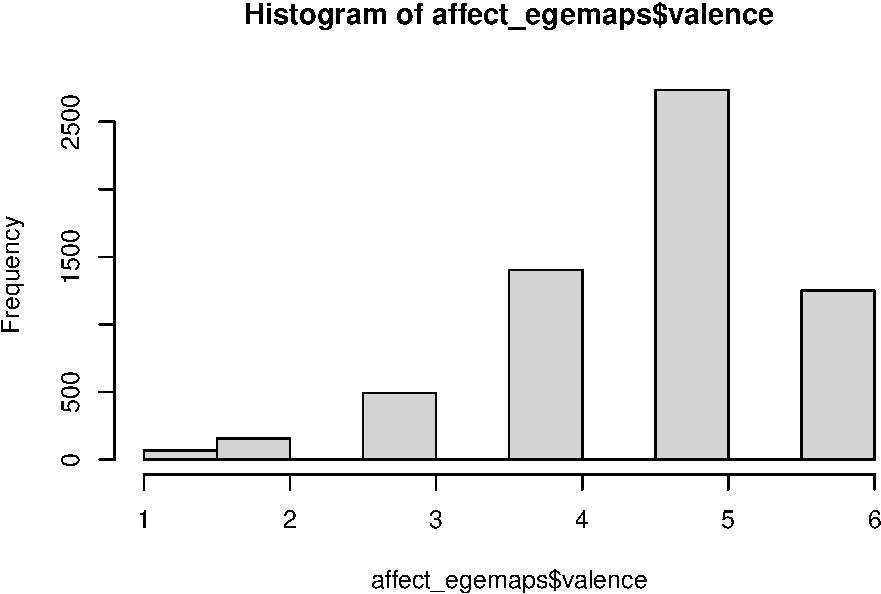
\includegraphics{AffectExperience_Audio_Manuscript_files/figure-latex/unnamed-chunk-2-1.pdf} 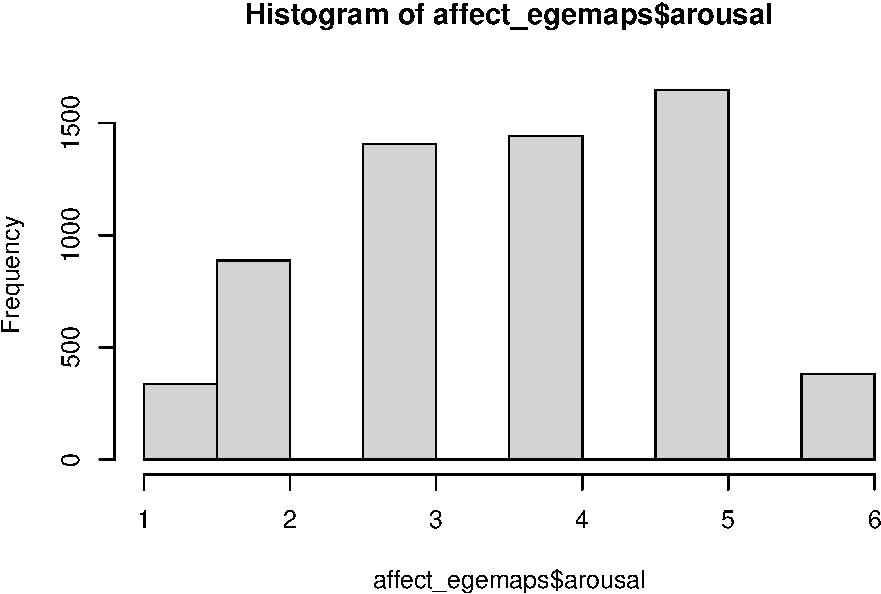
\includegraphics{AffectExperience_Audio_Manuscript_files/figure-latex/unnamed-chunk-2-2.pdf}

\hypertarget{predictive-modelling}{%
\subsection{Predictive Modelling}\label{predictive-modelling}}

We trained multiple supervised machine learning regression models on the extracted acoustic features for the prediction of self-reported valence and arousal. Here, we compared the predictive performance of Elastic Net regularized regression models (Zou \& Hastie, 2005) with those of a non-linear tree-based random forest model (Breiman, 2001; Wright \& Ziegler, 2017), and a baseline model. The baseline model would predict the respective mean values for valence and arousal of the respective training set for all cases in a test set. We evaluated the predictive performance of our models and tuned model hyperparameter in a nested cross-validation scheme (Bischl, Mersmann, Trautmann, \& Weihs, 2012). We blocked participants in the resampling procedure ensuring that for one train/test set pair the given participant is either in the training set or in the test set. We also ran the described analyses on the larger ComParE2016 feature set in order to investigate if a larger feature set improves predictions.This is relevant for potential application of affect recognition on device.

We evaluated the predictive performance of the models based on Spearman (rank) correlation (r) and mean absolute error (MAE) and between the predicted valence and arousal scores and participants' self-reported scores. To determine whether a model was predictive (alpha = 0.05) at all, we carried out t tests by comparing the MAE measures in all prediction models with those of the baseline models. We used variance corrected t tests based on 10-fold cross- validation to account for the dependence structure of cross-validation experiments (Nadeau \& Bengio, 2003). All comparisons were adjusted for multiple comparisons (n = 2) via Holm correction.

Further, for predictive models, we investigated which aspects of the voice contribute to the predictions. Therefore, we computed the grouped feature importance of the 25 Low Level Descriptors of the six parameters groups of the eGeMaps feature set (Au, Herbinger, Stachl, Bischl, \& Casalicchio, 2021).

All data processing and statistical analyses in this work were performed with the statistical software R version 4.0.2 (R Core Team, 2020). For machine learning, we used the mlr3 framework (Lang et al., 2019) and the DALEX package (Biecek, 2018). We provide the R code and our main figures in the project's repository of the Open Science Framework (OSF).

\hypertarget{results}{%
\section{Results}\label{results}}

\hypertarget{recognizing-valence-and-arousal-from-acoustic-voice-cues}{%
\subsection{Recognizing valence and arousal from acoustic voice cues}\label{recognizing-valence-and-arousal-from-acoustic-voice-cues}}

The employed algorithms significantly predicted valence and arousal above baseline levels.

For valence, neither the Random Forest models (r = 0.00, MAE = 0.82) nor the Elastic Net models (r = 0.02, MAE = 0.81) models did not predict significantly above baseline levels (r = NA, MAE = 0.81).

For arousal, neither the Random Forest models (r = 0.17, MAE = 1.10) nor the Elastic Net models (r = 0.12, MAE = 1.11) models did not predict significantly above baseline levels (r = NA, MAE = 1.12).

We compared prediction performance of algorithms trained on the smaller eGeMaPs (88 features) and the larger Compare2016 (6,000 features) feature sets. The larger Compare data

\hypertarget{predictiveness-of-acoustic-feature-groups}{%
\subsection{Predictiveness of acoustic feature groups}\label{predictiveness-of-acoustic-feature-groups}}

We identified predictive feature groups in valence and arousal predictions. For arousal, features related to loudness were most predictive. Show (grouped) feature importance for Low Level Descriptors (25). Show PDP plots for important feature groups. (Au, Herbinger, Stachl, Bischl, \& Casalicchio, 2021).

\hypertarget{model-diagnostics-and-semantics-effects-on-acoustics}{%
\subsection{Model diagnostics and semantics' effects on acoustics}\label{model-diagnostics-and-semantics-effects-on-acoustics}}

Our models were much more accurate in the middle and less accurate for extreme cases.
Our results indicate that semantics (i.e., the emotional content of the sentences) had not impact on predictions.

\begin{figure}
\centering
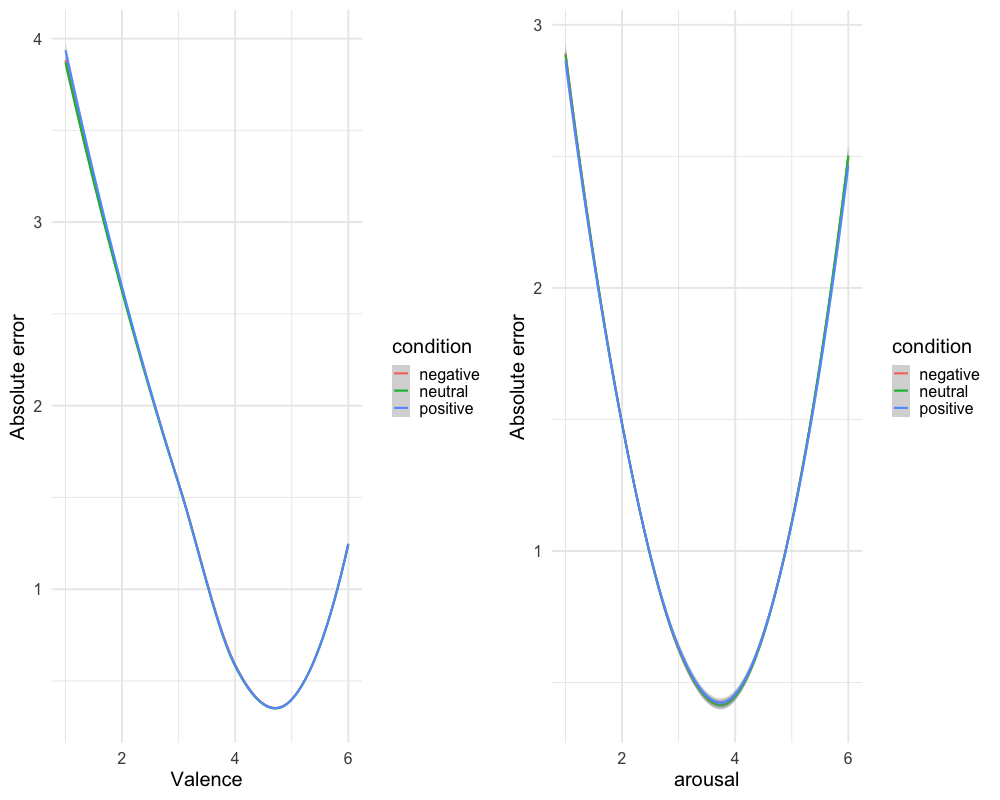
\includegraphics{../figures/performance_condtion.png}
\caption{Prediction performance for valence and arousal across sentence conditions. Predictions from Random Forest algorithm based on eGeMaPs features.}
\end{figure}

\hypertarget{discussion}{%
\section{Discussion}\label{discussion}}

We significantly predicted experienced self-reported arousal, but not valence, from voice cues collected in the wild using a novel smartphone-based privacy-respectful approach. We identified loudness and frequency to be particularly predictive of arousal. Our results suggest that semantics did not affect the recognition of affect experience from voice cues.

\hypertarget{recognizing-affect-experience-from-acoustic-voice-cues}{%
\subsection{Recognizing affect experience from acoustic voice cues}\label{recognizing-affect-experience-from-acoustic-voice-cues}}

Our results indicate that arousal experience can be automatically recognized from voice, where as valence experience cannot. Thereby, we report lower prediction performance than prior work on automatic prediction of affect expression (REF). Our findings that arousal can be recognized easier than valence is in line with prior research and theoretical considerations. Weidman and colleagues were unable to predict happiness, which could be interpreted as analogue to valence (Weidman et al., 2020). Valence is about the quality of affect, which is very individual.

We propose three reasons, why our predictive performance is lower than in prior work. First, our and prior research indicates that recognizing affect experience is more challenging than recognizing affect expression. Second, real-life affect is more difficult to recognized that enacted one (Vogt, André, \& Wagner, 2008). Third, there are less instances of extreme affect experiences in our data set compared to the data used in prior studies on acted emotions. We rather predicted mood, which is, by definition, less intense than emotion, which are short-lived and directed (\textbf{schererVocalCommunicationEmotion2003?}).

\hypertarget{semantics-had-no-impact-on-affect-recognition-from-acoustics}{%
\subsection{Semantics had no impact on affect recognition from acoustics}\label{semantics-had-no-impact-on-affect-recognition-from-acoustics}}

Our results based on a novel experimental design suggest that the semantics, meaning the content what participants talked about, did not have an impact on affect recognition. This implies that it does not matter what people talk about when inferring affect experience from voice.

\hypertarget{economic-on-device-acoustic-feature-extraction}{%
\subsection{Economic on-device acoustic feature extraction}\label{economic-on-device-acoustic-feature-extraction}}

Previously, researchers were limited in the available methods to collect in-situ self-report on affect experience and corresponding voice samples. The only two viable solution, were using the EAR and having participants make audio records using their smartphones and e-mailing files to researchers. We introduced a novel, privacy-pervasive framework combining ESM and on-device acoustic feature extraction with many advantages. Further, in line with prior research (Weidman et al., 2020), our results suggest that a sparse

We show that sparse feature extraction on the device is fruitful and privacy-preserving. This could be used as diagnostics instrument. Our findings indicate that more features do not lead to more accurate predictions. Small features set is less computationally expensive and would allow for online or on-device pre-processing in a scientific or applied setting.

\hypertarget{implications}{%
\subsection{Implications}\label{implications}}

Our results suggest that subjective affect experience, particularly valence, is much more difficult to recognize than affect expression. By making our predictions interpretable we added to affect and voice theory.

Further, our new research approach to collect voice data offers a fruitful avenue for future research based on voice data. It also offers in the sense of goal, experimental variation of sentences : use smartphone as experimental lab (Miller, 2012). We also show that an economic acoustic feature set sufficient, this is relevant for application.

Our findings have broad implications for the monitoring of affect experience in a practical setting. They question the proclaimed performance of commercial affect recognition algorithms and highlight the challenges ahead in affect monitoring, for example in mental health care. Current expectations, particularly of commercial solutions for affect predictions from voice, might be overoptimistic. Finally, implications for the privacy of users of, for example, voice assistants. No impact of semantics on affect recognition

\hypertarget{limitations-and-future-directions}{%
\subsection{Limitations and future directions}\label{limitations-and-future-directions}}

The main limitations of our work lie in our privacy-preserving on-device voice recording approach. In contrast to other studies, we extracted acoustic features directly on participants' smartphones instead of transferring raw audio records to our servers for further analyses. As a consequence, we have no opportunity to check if participants truly complied with study instructions and had recorded their voice while reading out the predefined sentences accordingly. Further, our approach did not allow to control for records' background noise (e.g., when participants were outside next to a road).

While the predefined sentences allowed us to control for the semantics of what participants talked about in their voice records we let them record, they we unable to express themselves freely. Possibly, if participants were allowed to talk about a topic of their choice, their affect experience would have manifested more strongly in their voice learning to more accurate predictions. In future studies, participants could be free with regard to the content they can talk about and pre-trained language models extract features of what they talk about (e.g., specific topics) directly on the device, too. Thereby, there would be no raw data transferred, but potentially valuable information of language content could be also used for affect recognition.

Because we collected in-situ self reports of affect experience from participants' everyday life, most of our data represents average affect experience and much fewer extreme cases. This, however, represents the normal everyday states of regular people, for whom many of the affect recognition algorithms were designed. Possibly, if future studies are able to collect more data from extreme cases, such as from clinical samples, results could be more distinct.

Moreover, future work should further account for the subjective nature of affect experience, particularly valence, by investigating within-person fluctuations of affect experience and speech acoustics. Potentially, researchers could create idiosyncratic (person-specific) models that are trained on data of a single participant. Finally, extracted information from voice could be merged with other sensing data (e.g., movement patterns) into one model to improve predictions.

\hypertarget{conclusion}{%
\section{Conclusion}\label{conclusion}}

In this work, we made predictions based on voice parameters collected in the wild using smartphones. We used a privacy protective on-device feature extraction. Our models predicted arousal significantly above baseline levels, but not arousal. Further, we investigated the effects of semantics on prosody in affect recognition. We discussed implications for theory and practice and further research opportunities.

\newpage

\hypertarget{references}{%
\section{References}\label{references}}

\begingroup
\setlength{\parindent}{-0.5in}
\setlength{\leftskip}{0.5in}

\hypertarget{refs}{}
\begin{CSLReferences}{1}{0}
\leavevmode\hypertarget{ref-auGroupedFeatureImportance2021}{}%
Au, Q., Herbinger, J., Stachl, C., Bischl, B., \& Casalicchio, G. (2021). \emph{Grouped {Feature Importance} and {Combined Features Effect Plot}}.

\leavevmode\hypertarget{ref-ben-davidboazm.ProsodySemanticsAre2016}{}%
Ben-David Boaz M., Multani Namita, Shakuf Vered, Rudzicz Frank, \& van Lieshout Pascal H. H. M. (2016). Prosody and {Semantics Are Separate} but {Not Separable Channels} in the {Perception} of {Emotional Speech}: Test for {Rating} of {Emotions} in {Speech}. \emph{Journal of Speech, Language, and Hearing Research}, \emph{59}(1), 72--89. \url{https://doi.org/10.1044/2015_JSLHR-H-14-0323}

\leavevmode\hypertarget{ref-biecekDALEXExplainersComplex2018}{}%
Biecek, P. (2018). {DALEX}: Explainers for {Complex Predictive Models} in {R}. \emph{Journal of Machine Learning Research}, \emph{19}(84), 1--5.

\leavevmode\hypertarget{ref-bischlResamplingMethodsMetaModel2012}{}%
Bischl, B., Mersmann, O., Trautmann, H., \& Weihs, C. (2012). Resampling {Methods} for {Meta}-{Model Validation} with {Recommendations} for {Evolutionary Computation}. \emph{Evolutionary Computation}, \emph{20}(2), 249--275. \url{https://doi.org/10.1162/EVCO_a_00069}

\leavevmode\hypertarget{ref-breimanRandomForests2001}{}%
Breiman, L. (2001). Random forests. \emph{Machine Learning}, \emph{45}(1), 5--32.

\leavevmode\hypertarget{ref-defrenEmotionalSpeechPerception2018}{}%
Defren, S., de Brito Castilho Wesseling, P., Allen, S., Shakuf, V., Ben-David, B., \& Lachmann, T. (2018). Emotional {Speech Perception}: A set of semantically validated {German} neutral and emotionally affective sentences. In \emph{9th {International Conference} on {Speech Prosody} 2018} (pp. 714--718). {ISCA}. \url{https://doi.org/10.21437/SpeechProsody.2018-145}

\leavevmode\hypertarget{ref-demetriouSelfReportQuestionnaires2015}{}%
Demetriou, C., Ozer, B. U., \& Essau, C. A. (2015). Self-{Report Questionnaires}. In R. L. Cautin \& S. O. Lilienfeld (Eds.), \emph{The {Encyclopedia} of {Clinical Psychology}} (pp. 1--6). {Hoboken, NJ, USA}: {John Wiley \& Sons, Inc.} \url{https://doi.org/10.1002/9781118625392.wbecp507}

\leavevmode\hypertarget{ref-dukesRiseAffectivism2021}{}%
Dukes, D., Abrams, K., Adolphs, R., Ahmed, M. E., Beatty, A., Berridge, K. C., \ldots{} Sander, D. (2021). The rise of affectivism. \emph{Nature Human Behaviour}, 1--5. \url{https://doi.org/10.1038/s41562-021-01130-8}

\leavevmode\hypertarget{ref-eybenGenevaMinimalisticAcoustic2016}{}%
Eyben, F., Scherer, K. R., Schuller, B. W., Sundberg, J., Andre, E., Busso, C., \ldots{} Truong, K. P. (2016). The {Geneva Minimalistic Acoustic Parameter Set} ({GeMAPS}) for {Voice Research} and {Affective Computing}. \emph{IEEE Transactions on Affective Computing}, \emph{7}(2), 190--202. \url{https://doi.org/10.1109/TAFFC.2015.2457417}

\leavevmode\hypertarget{ref-kassamEffectsMeasuringEmotion2013}{}%
Kassam, K. S., \& Mendes, W. B. (2013). The effects of measuring emotion: Physiological reactions to emotional situations depend on whether someone is asking. \emph{PloS One}, \emph{8}(7), e64959. \url{https://doi.org/10.1371/journal.pone.0064959}

\leavevmode\hypertarget{ref-knightAmazonWorkingMaking2016a}{}%
Knight, W. (2016). Amazon {Working} on {Making Alexa Recognize Your Emotions}. \emph{MIT Technology Review}. https://www.technologyreview.com/2016/06/13/159665/amazon-working-on-making-alexa-recognize-your-emotions/.

\leavevmode\hypertarget{ref-kuppensFeelingsChangeAccounting2010}{}%
Kuppens, P., Oravecz, Z., \& Tuerlinckx, F. (2010). Feelings change: Accounting for individual differences in the temporal dynamics of affect. \emph{Journal of Personality and Social Psychology}, \emph{99}(6), 1042--1060. \url{https://doi.org/10.1037/a0020962}

\leavevmode\hypertarget{ref-langMlr3ModernObjectoriented2019}{}%
Lang, M., Binder, M., Richter, J., Schratz, P., Pfisterer, F., Coors, S., \ldots{} Bischl, B. (2019). Mlr3: A modern object-oriented machine learning framework in {R}. \emph{Journal of Open Source Software}, \emph{4}(44), 1903. \url{https://doi.org/10.21105/joss.01903}

\leavevmode\hypertarget{ref-linyiProsodyDominatesSemantics2020}{}%
Lin Yi, Ding Hongwei, \& Zhang Yang. (2020). Prosody {Dominates Over Semantics} in {Emotion Word Processing}: Evidence {From Cross}-{Channel} and {Cross}-{Modal Stroop Effects}. \emph{Journal of Speech, Language, and Hearing Research}, \emph{63}(3), 896--912. \url{https://doi.org/10.1044/2020_JSLHR-19-00258}

\leavevmode\hypertarget{ref-mandellSpotifyPatentsVoice2020}{}%
Mandell, J. (2020). Spotify {Patents A Voice Assistant That Can Read Your Emotions}. \emph{Forbes}. https://www.forbes.com/sites/joshmandell/2020/03/12/spotify-patents-a-voice-assistant--that-can-read-your-emotions/.

\leavevmode\hypertarget{ref-mehlElectronicallyActivatedRecorder2017}{}%
Mehl, M. R. (2017). The {Electronically Activated Recorder} ({EAR}): A {Method} for the {Naturalistic Observation} of {Daily Social Behavior}. \emph{Current Directions in Psychological Science}, \emph{26}(2), 184--190. \url{https://doi.org/10.1177/0963721416680611}

\leavevmode\hypertarget{ref-millerSmartphonePsychologyManifesto2012}{}%
Miller, G. (2012). The {Smartphone Psychology Manifesto}. \emph{Perspectives on Psychological Science: A Journal of the Association for Psychological Science}, \emph{7}(3), 221--237. \url{https://doi.org/10.1177/1745691612441215}

\leavevmode\hypertarget{ref-molnarInterpretableMachineLearning2019}{}%
Molnar, C. (2019). \emph{Interpretable {Machine Learning}}.

\leavevmode\hypertarget{ref-muaremiAssessingBipolarEpisodes2014}{}%
Muaremi, A., Gravenhorst, F., Grünerbl, A., Arnrich, B., \& Tröster, G. (2014). \emph{Assessing {Bipolar Episodes Using Speech Cues Derived} from {Phone Calls}}. \emph{Lecture Notes of the Institute for Computer Sciences, Social-Informatics and Telecommunications Engineering, LNICST} (Vol. 100). \url{https://doi.org/10.1007/978-3-319-11564-1_11}

\leavevmode\hypertarget{ref-nadeauInferenceGeneralizationError2003}{}%
Nadeau, C., \& Bengio, Y. (2003). Inference for the {Generalization Error}. \emph{Machine Learning}, \emph{52}(3), 239--281. \url{https://doi.org/10.1023/A:1024068626366}

\leavevmode\hypertarget{ref-schoedelBasicProtocolSmartphone2020}{}%
Schoedel, R., \& Oldemeier, M. (2020). Basic {Protocol}: Smartphone {Sensing Panel Study}. \url{https://doi.org/10.23668/psycharchives.2901}

\leavevmode\hypertarget{ref-schullerVoiceSpeechAnalysis2011}{}%
Schuller, B. (2011). Voice and {Speech Analysis} in {Search} of {States} and {Traits}. In A. A. Salah \& T. Gevers (Eds.), \emph{Computer {Analysis} of {Human Behavior}} (pp. 227--253). {London}: {Springer London}. \url{https://doi.org/10.1007/978-0-85729-994-9_9}

\leavevmode\hypertarget{ref-schullerSpeechEmotionRecognition2018}{}%
Schuller, B. (2018). Speech emotion recognition: Two decades in a nutshell, benchmarks, and ongoing trends. \emph{Communications of the ACM}, \emph{61}(5), 90--99. \url{https://doi.org/10.1145/3129340}

\leavevmode\hypertarget{ref-schullerRecognisingRealisticEmotions2011}{}%
Schuller, B., Batliner, A., Steidl, S., \& Seppi, D. (2011). Recognising realistic emotions and affect in speech: State of the art and lessons learnt from the first challenge. \emph{Speech Communication}, \emph{53}(9), 1062--1087. \url{https://doi.org/10.1016/j.specom.2011.01.011}

\leavevmode\hypertarget{ref-schullerINTERSPEECH2016Computational2016}{}%
Schuller, B., Steidl, S., Batliner, A., Hirschberg, J., Burgoon, J., Baird, A., \ldots{} Evanini, K. (2016). \emph{The {INTERSPEECH} 2016 {Computational Paralinguistics Challenge}: Deception, {Sincerity} and {Native Language}} (p. 2005). \url{https://doi.org/10.21437/Interspeech.2016-129}

\leavevmode\hypertarget{ref-sunLanguageWellbeingTracking2020}{}%
Sun, J., Schwartz, H. A., Son, Y., Kern, M. L., \& Vazire, S. (2020). The language of well-being: Tracking fluctuations in emotion experience through everyday speech. \emph{Journal of Personality and Social Psychology}, \emph{118}(2), 364--387. \url{https://doi.org/10.1037/pspp0000244}

\leavevmode\hypertarget{ref-vogtAutomaticRecognitionEmotions2008}{}%
Vogt, T., André, E., \& Wagner, J. (2008). Automatic {Recognition} of {Emotions} from {Speech}: A {Review} of the {Literature} and {Recommendations} for {Practical Realisation}. In C. Peter \& R. Beale (Eds.), \emph{Affect and {Emotion} in {Human}-{Computer Interaction}} (Vol. 4868, pp. 75--91). {Berlin, Heidelberg}: {Springer Berlin Heidelberg}. \url{https://doi.org/10.1007/978-3-540-85099-1_7}

\leavevmode\hypertarget{ref-wangStudentLifeAssessingMental2014}{}%
Wang, R., Chen, F., Chen, Z., Li, T., Harari, G., Tignor, S., \ldots{} Campbell, A. T. (2014). {StudentLife}: Assessing mental health, academic performance and behavioral trends of college students using smartphones. In \emph{Proceedings of the 2014 {ACM International Joint Conference} on {Pervasive} and {Ubiquitous Computing}} (pp. 3--14). {Seattle Washington}: {ACM}. \url{https://doi.org/10.1145/2632048.2632054}

\leavevmode\hypertarget{ref-weidmanNotHearingHappiness2020}{}%
Weidman, A. C., Sun, J., Vazire, S., Quoidbach, J., Ungar, L. H., \& Dunn, E. W. (2020). ({Not}) hearing happiness: Predicting fluctuations in happy mood from acoustic cues using machine learning. \emph{Emotion (Washington, D.C.)}, \emph{20}(4), 642--658. \url{https://doi.org/10.1037/emo0000571}

\leavevmode\hypertarget{ref-weningerAcousticsEmotionAudio2013}{}%
Weninger, F., Eyben, F., Schuller, B. W., Mortillaro, M., \& Scherer, K. R. (2013). On the {Acoustics} of {Emotion} in {Audio}: What {Speech}, {Music}, and {Sound} have in {Common}. \emph{Frontiers in Psychology}, \emph{4}. \url{https://doi.org/10.3389/fpsyg.2013.00292}

\leavevmode\hypertarget{ref-wiltingRealVsActed2006}{}%
Wilting, J., Krahmer, E. J., \& Swerts, M. G. J. (2006). Real vs. Acted emotional speech. \emph{Proceedings of the International Conference on Spoken Language Processing (Interspeech 2006)}.

\leavevmode\hypertarget{ref-wrightRangerFastImplementation2017}{}%
Wright, M. N., \& Ziegler, A. (2017). Ranger: A {Fast Implementation} of {Random Forests} for {High Dimensional Data} in {C}++ and {R}. \emph{Journal of Statistical Software}, \emph{77}(1), 1--17. \url{https://doi.org/10.18637/jss.v077.i01}

\leavevmode\hypertarget{ref-zouRegularizationVariableSelection2005}{}%
Zou, H., \& Hastie, T. (2005). Regularization and variable selection via the elastic net. \emph{Journal of the Royal Statistical Society: Series B (Statistical Methodology)}, \emph{67}(2), 301--320. \url{https://doi.org/10.1111/j.1467-9868.2005.00503.x}

\end{CSLReferences}

\endgroup


\end{document}
